% Welcome! This is the Category Capital Beamer Template. This work, "Category Capital Beamer Theme," is a derivative of the unofficial Integrated Mill Systems Beamer Template, which work ("Integrated Mill Systems Beamer Theme", licensed under CC 4.0) is itself a derivative of "Umeå University Unofficial Beamer Theme" by Jesper Erixon, CC 4.0 BY.
% (https://www.overleaf.com/latex/templates/umea-university-unofficial-beamer-theme/ptvmzxqzjhcn)
% which is a derivative
% of "University of Udine Unofficial Beamer Theme" by Marco Basaldella, University of Udine, CC 4.0 BY. 
% (https://www.overleaf.com/latex/templates/university-of-udine-unofficial-beamer-theme/zndkgxrjsdzt) 
%
% The main functionality and commands are 
% all credited to Marco Basaldella (and Till Tantau et al. for creating the beamer document class in
% the first place).  
%
% "Category Capital Beamer Theme" is licensed under CC 4.0 by Steve Huntsman. All logos are copyright Category Capital: all rights reserved.

% Background photo taked by 
% Chris Liverani (https://unsplash.com/@chrisliverani?utm_source=unsplash&utm_medium=referral&utm_content=creditCopyText)
% on Unsplash (https://unsplash.com/s/photos/header-industrial?utm_source=unsplash&utm_medium=referral&utm_content=creditCopyText) 


% Note that [usenames,dvipsnames] is MANDATORY due to compatibility
% issues between tikz and xcolor packages.

\documentclass[usenames,dvipsnames,10pt,aspectratio=169]{beamer} 
% Add option 'aspectratio=169' for 16:9 widescreen 
% Add option  'handout' to ignore animations
% If you have a smaller amount of text, feel free to also try '11pt'! / Jesper

\usepackage[utf8]{inputenc}
\usepackage{verbatim}
\usetheme{ims}

%%% Bibliography
\usepackage[style=authoryear,backend=biber]{biblatex}
\addbibresource{bibliography.bib}

% Author names in publication list are consistent 
% i.e. name1 surname1, name2 surname2
% See https://tex.stackexchange.com/questions/106914/biblatex-does-not-reverse-the-first-and-last-names-of-the-second-author
\DeclareNameAlias{author}{given-family}

%%% Suppress biblatex annoying warning
\usepackage{silence}
\WarningFilter{biblatex}{Patching footnotes failed}

% Misc packages
\usepackage{tikz} % drawing
\usepackage[all]{xy}
\usetikzlibrary{arrows,shapes}

%%% Some useful commands
% pdf-friendly newline in links
\newcommand{\pdfnewline}{\texorpdfstring{\newline}{ }} 
% Fill the vertical space in a slide (to put text at the bottom)
\newcommand{\framefill}{\vskip0pt plus 1filll}

%%% Additional packages, added by Jesper Erixon
% Use babel to neatly translate 'abstract' etc. to swedish  or other supported language
%\usepackage[swedish]{babel}

%%% Enter additional packages below (or above, I can't stop you)! / Jesper
\renewcommand{\proofname}{\sffamily{Proof}}

%%%%%%%%%%%%%%%%%%%%%%%%%%%%%%%%%%%%%%%%%%%%%%%%%%%%%%%%%%%%%%%%%%%%%%%%%%%%%%%%%%%%%
%%%%%%%%%%%%%%%%%%%%%%%%%%%%%%% YOUR PRESENTATION BELOW %%%%%%%%%%%%%%%%%%%%%%%%%%%%%
%%%%%%%%%%%%%%%%%%%%%%%%%%%%%%%%%%%%%%%%%%%%%%%%%%%%%%%%%%%%%%%%%%%%%%%%%%%%%%%%%%%%%
\title[Category Capital Beamer Theme]{ \ \\ \ \\ Prospects for applications of magnitude homology}
\date{July 2023}
%\date[\today]{\small\today}
\author[Steve Huntsman]{ \ \pdfnewline \ \pdfnewline \pdfnewline \pdfnewline \pdfnewline  
  Steve Huntsman  \pdfnewline
  %\texttt{sch213@nyu.edu}
}
\institute{SIAM AG / Applications of Magnitude and Magnitude Homology to Network Analysis} 

\begin{document}


{
\setbeamercolor{background canvas}{bg=CatCapBlue}
\begin{frame}
\titlepage
\end{frame}
}

\begin{frame}{\contentsname}
\tableofcontents
\end{frame}


\section{{\bf Context} from mainstream topological data analysis to discrete tools}

\begin{frame}{Mainstream TDA has a playbook}
		\begin{itemize}
			\item {\color{CatCapGold}Approximate} $\{X_j\}_{j=1}^n \subset (\mathbb{R}^d)^n$ at various scales
			\item {\color{CatCapGold}Compute} a topological invariant of each approximation
			\item {\color{CatCapGold}Highlight} invariants that persist across scales
			\item E.g., 12 equispaced points on the unit circle (half-distance $\Delta \approx 0.2588$)
			\begin{itemize}
				\item $\beta_0 = 12 \cdot 1_{[0,\Delta)} + 1_{[\Delta,1)} + 1_{[1,\infty)}$
				\item $\beta_1 = {\color{white}12 \cdot 1_{[0,\Delta)} + {\color{black}1_{[\Delta,1)}}}$
			\end{itemize}
		\end{itemize}
		\begin{center}
			\begin{tikzpicture}[->,>=stealth',shorten >=1pt]
				\coordinate (x00) at (1.0000,0);
				\coordinate (x01) at (0.8660,0.5000);
				\coordinate (x02) at (0.5000,0.8660);
				\coordinate (x03) at (0.0000,1.0000);
				\coordinate (x04) at (-0.5000,0.8660);
				\coordinate (x05) at (-0.8660,0.5000);
				\coordinate (x06) at (-1.0000,0.0000);
				\coordinate (x07) at (-0.8660,-0.5000);
				\coordinate (x08) at (-0.5000,-0.8660);
				\coordinate (x09) at (-0.0000,-1.0000);
				\coordinate (x10) at (0.5000,-0.8660);
				\coordinate (x11) at (0.8660,-0.5000);
				\foreach \x in {
					x00,x01,x02,x03,x04,x05,x06,x07,x08,x09,x10,x11}
					\draw [fill,CatCapBlue,opacity=0.25] (\x) circle [radius=0.2];
				\foreach \x in {
					x00,x01,x02,x03,x04,x05,x06,x07,x08,x09,x10,x11}
					\draw [fill] (\x) circle [radius=0.025];
				\node (z) at (0,0) {scale $0.2$};
				\draw [opacity=0] (-1,0) circle [radius=0.3];
				\draw [opacity=0] (1,0) circle [radius=0.3];
				\draw [opacity=0] (0,-1) circle [radius=0.3];
				\draw [opacity=0] (0,1) circle [radius=0.3];
			\end{tikzpicture}
			\begin{tikzpicture}[->,>=stealth',shorten >=1pt]
				\coordinate (x00) at (1.0000,0);
				\coordinate (x01) at (0.8660,0.5000);
				\coordinate (x02) at (0.5000,0.8660);
				\coordinate (x03) at (0.0000,1.0000);
				\coordinate (x04) at (-0.5000,0.8660);
				\coordinate (x05) at (-0.8660,0.5000);
				\coordinate (x06) at (-1.0000,0.0000);
				\coordinate (x07) at (-0.8660,-0.5000);
				\coordinate (x08) at (-0.5000,-0.8660);
				\coordinate (x09) at (-0.0000,-1.0000);
				\coordinate (x10) at (0.5000,-0.8660);
				\coordinate (x11) at (0.8660,-0.5000);
				\foreach \x in {
					x00,x01,x02,x03,x04,x05,x06,x07,x08,x09,x10,x11}
					\draw [fill,CatCapGold,opacity=0.5] (\x) circle [radius=0.3];
				\foreach \x in {
					x00,x01,x02,x03,x04,x05,x06,x07,x08,x09,x10,x11}
					\draw [fill] (\x) circle [radius=0.025];
				\node (z) at (0,0) {scale $0.3$};
				\draw [opacity=0] (-1,0) circle [radius=0.2];
				\draw [opacity=0] (1,0) circle [radius=0.2];
				\draw [opacity=0] (0,-1) circle [radius=0.2];
				\draw [opacity=0] (0,1) circle [radius=0.2];
			\end{tikzpicture}
			\begin{tikzpicture}[->,>=stealth',shorten >=1pt]
				\clip (-2.1,-1.3) rectangle (2.1,1.3);		
				\coordinate (x00) at (1.0000,0);
				\coordinate (x01) at (0.8660,0.5000);
				\coordinate (x02) at (0.5000,0.8660);
				\coordinate (x03) at (0.0000,1.0000);
				\coordinate (x04) at (-0.5000,0.8660);
				\coordinate (x05) at (-0.8660,0.5000);
				\coordinate (x06) at (-1.0000,0.0000);
				\coordinate (x07) at (-0.8660,-0.5000);
				\coordinate (x08) at (-0.5000,-0.8660);
				\coordinate (x09) at (-0.0000,-1.0000);
				\coordinate (x10) at (0.5000,-0.8660);
				\coordinate (x11) at (0.8660,-0.5000);
				\foreach \x in {
					x00,x01,x02,x03,x04,x05,x06,x07,x08,x09,x10,x11}
					\draw [fill,CatCapSilver,opacity=0.25] (\x) circle [radius=1.1];
				\foreach \x in {
					x00,x01,x02,x03,x04,x05,x06,x07,x08,x09,x10,x11}
					\draw [fill] (\x) circle [radius=0.025];
				\node (z) at (0,0) {scale $1.1$};
				\draw [opacity=0] (-1,0) circle [radius=0.2];
				\draw [opacity=0] (1,0) circle [radius=0.2];
				\draw [opacity=0] (0,-1) circle [radius=0.2];
				\draw [opacity=0] (0,1) circle [radius=0.2];
			\end{tikzpicture}
		\end{center}
\end{frame}


\begin{frame}{We are going to play a simpler game}
	\begin{itemize}
		\item<1-> Data that interests us is fundamentally discrete
		\begin{itemize}
			\item<1-> {\color{CatCapGold}Approximate} {\bf nothing} (via representation or model if need be)
			\item<1-> {\color{CatCapGold}Compute} a (co)chain complex {\bf directly from the data}: simplicial complexes are optional technical devices
			\item<1-> {\color{CatCapGold}Highlight} any persistence {\bf incidentally}: it often won't apply
		\end{itemize}
		\item<2-> Archetype: Dowker homology
		\begin{itemize}
			\item<2-> Relation corresponds to a pair of homotopy equivalent simplicial complexes
			\item<2-> $\mathbb{F}_2$ homology readily computed directly from relation itself, without ever constructing either simplicial complex
		\end{itemize}
		\item<3-> Many well known discrete tools are underutilized
		\begin{itemize}
			\item<3-> Finite topological spaces \emph{per se}
			\item<3-> Simplicial complexes generated by posets/hypergraphs
			\item<3-> Discrete Morse theory
			\item<3-> \dots
		\end{itemize}
	\end{itemize}
\end{frame}

\begin{frame}{This simpler game has practical relevance}
	\begin{itemize}
		\item<1-> Dowker applications:
		\begin{itemize}
			\item<1-> Witness complexes
			\item<1-> Systems/sociology
			\item<1-> Robotics
			\item<1-> Neuroscience
			\item<1-> Privacy
			\item<1-> Software engineering 
			\item<1-> \dots
			\item<1-> Exercises for audience: cyber interactions like user/computer; process/file; etc
		\end{itemize}
		\item<2-> Magnitude homology for digraphs is suited for novel applications\dots
		\begin{itemize}
			\item<2-> \dots that can give rise to new capabilities
			\item<3-> Cf. path homology, which is related but lacks \emph{ab initio} source/target specificity
		\end{itemize}
	\end{itemize}
\end{frame}


\section{{\bf Magnitude homology} with the briefest nod towards cyber applications}

\begin{frame}{Magnitude homology is readily constructed}
	\begin{itemize}
		\item<1-> Let $(X,d)$ be a Lawvere metric space $\Leftrightarrow d =$ extended quasipseudometric
		\begin{itemize}
			\item<1-> $d : X \times X \rightarrow [0,\infty]$ \hfill (extended)
			\item<1-> $d$ need not be symmetric \hfill (quasi-)
			\item<1-> $d(x,x)$ need not be zero \hfill (pseudo-)
			\item<1-> $(X,d)$ best thought of here as a category enriched over the poset $([0,\infty],\ge)$
		\end{itemize}
		\item<2-> A \emph{$k$-simplex} in $X$ is an ordered tuple $x^{(k)} := (x_0,\dots,x_k) \in X^{k+1}$ s.t. $x_j \ne x_{j-1}$ %for $j \in [k]$ 
		\item<2-> The \emph{length} of $x^{(k)}$ is $\lambda(x^{(k)}) := \sum_{j=1}^k d(x_{j-1},x_j)$
	\end{itemize}
	\begin{block}<3-> {The $\mathbb{R}$-graded \emph{magnitude chain complex} (as before $R$ is a coefficient ring):}
		 \begin{itemize}
		 	\item $k$-chains: $MC_{k,L}(X) := R \left \{ x^{(k)} \text{ a $k$-simplex in $X$} : \lambda(x^{(k)}) = L \right \}$
			\item differential: $\partial_k : MC_{k,L}(X) \rightarrow MC_{k-1,L}(X)$ given by $\partial_k := \sum_{j=1}^{k-1} (-1)^j \partial^{(j)}$
			\begin{itemize}
				\item $\partial^{(j)}(x^{(k)}) := \nabla_j x^{(k)} \text{ if } d(x_{j-1},x_{j+1}) = d(x_{j-1},x_j) + d(x_j,x_{j+1})$ and $:= 0 \text{ otherwise}$
				% \item As before $\nabla_j$ acts on a tuple by deleting the corresponding entry
			\end{itemize}
			\item Appropriate notion of chain map is induced by $d$-nonincreasing maps
		 \end{itemize} 
	\end{block}
	\begin{alertblock}<4-> {The \emph{magnitude homology} of $X$\dots}
		\dots is the homology of the magnitude chain complex
	\end{alertblock} 
\end{frame}

\begin{frame}{MH has attractive features}
	\begin{itemize}
		\item<1-> For a digraph $D$, there is a decomposition of the form $$MC_{\bullet,L}(D) = \bigoplus_{s,t \in V(D)} MC_{\bullet,L}^{(s,t)}(D)$$
		\begin{itemize}
			\item<1-> $MC_{\bullet,L}^{(s,t)}(D)$ generated by simplices with (initial, terminal) entries $(s,t)$
			\item<2-> This structure makes MH particularly convenient for unweighted digraphs
		\end{itemize}
		\item<3-> A ``blurred'' variant replaces $\lambda = L$ in the chain complex definition with $\lambda \le L$
		\item<4-> MH is related to both persistent homology and path homology
		\item<5-> \emph{Magnitude cohomology} has an analogue of the cup product
		\begin{itemize}
			\item<5-> Ring structure determines the space for finite extended quasi-metric spaces 
			\begin{itemize}
				\item<5-> E.g., digraphs; finite metric spaces
			\end{itemize}
			\item<5-> Meanwhile, tree magnitude (co)homology \emph{groups} only depend on \#(vertices)
		\end{itemize} 
	\end{itemize}
\end{frame}

\begin{frame}{MH generalizes to enriched categories}
	\begin{itemize}
		\item Consider enriched category of sub-flow graphs of a given flow graph
		\begin{itemize}
			\item For semicartesianness, take a specific category $\mathbf{F}$ of ``two-terminal graphs''
            		\begin{itemize}
            			\item Presents some technical issues for decomposition (probably surmountable)
            		\end{itemize}
            		\item The topological entropy is a ``size function'' over the max-plus semiring
            		\begin{itemize}
            			\item Recall this is log rate of growth of possible paths as a function of length
            		\end{itemize}
            		\item This setup dovetails with the source-target direct sum decomposition
            		\item A categorification might be interesting and efficiently computable
            		\begin{itemize}
            			\item Representatives might encode nice structure
            		\end{itemize}
            		\item Possibility to connect to useful cyber applications via compilers
		\end{itemize}
		\item More ambitiously, consider $\mathbf{F} \times \mathbf{M}$ where $\mathbf{M}$ is a  ``matrix category'' of data
		\begin{itemize}
			\item Size function may be something like the zeta function of a Markov chain
		\end{itemize}
		\item Suitable data obtainable from program analysis
		\begin{itemize}
			\item Simpler initial goal: use hitting probabilities metric of Boyd \emph{et al.} (this is vanilla)
		\end{itemize}
	\end{itemize}
\end{frame}


%An interesting if still speculative possibility for deeper applications to processes, computer programs, etc. is to consider categories of the form $\mathbf{F} \times \mathbf{M}$ where $\mathbf{F}$ is a suitable category of ``flow-like'' digraphs that have single inputs and outputs and $\mathbf{M}$ is a suitable category of data (perhaps scalar if not in the spirit of a nondegenerate matrix category). The monoidal structure on $\mathbf{F}$ is simply gluing the output of one `flow-like'' digraph to the input of another along the lines of \cite{huntsman2022magnitude}. That is, each ``flow-like'' graph has associated data that compose nicely under series composition. A specific instantiation of $\mathbf{F}$ that is algorithmically and categorically well-behaved (in particular, semicartesian) is likely obtainable via minor technical modifications to the notion of a \emph{two-terminal graph} \cite{vanhatalo2008refined}.
%
%In order to have a useful notion of magnitude in this context, it is necessary to have a size function (or for magnitude homology \cite{leinster2021magnitude}, a strong symmetric monoidal functor from a semicartesian symmetric monoidal category to a suitable abelian symmetric monoidal category) that consolidates the graphical and matrix data. A good candidate for constructing something in this vein appears to be the zeta function of a finite Markov chain \cite{parry1977block} that encodes (e.g.) graph traversal probabilities.



\section{{\bf Examples} in the vein of neural stuff (feedforward nets and actual brains)}


\begin{frame}{MH measures nonconvexity}

    %n = 2;
    %p = 2;
    %foo = diag(ones(1,(n-2)*p+2),p); 
    %foo(1,2:(p+1)) = 1; % last of these is redundant per above
    %foo(((n-2)*p+2):((n-1)*p+1),(n-1)*p+2) = 1;
    %%
    %% figure; plot(digraph(foo));
    %blur = 0;
    %eulerian = 0;
    %[allReps,betti,~,~,~,~,~] = magnitudeHomology(digraph(foo),n+1,blur,eulerian);
    %%
    %bar = allReps{1,size(allReps,2)}{3,n+1}

\begin{alertblock}{Let $P_{p,n}$ be the DAG formed from $p$ parallel paths of $n$ arcs from $1$ to  $(n-1)p+2$}
Then all the Betti numbers are zero except for $$\beta(P_{p,n})_{0,0} = |V(P_{p,n})| = (n-1)p+2;$$ $$\beta(P_{p,n})_{1,1} = |A(P_{p,n})| = np,$$ and $$\beta(P_{p,n})_{2,n} = p-1;$$ i.e., there are $p-1$ ``convexity defects'' of length $n$ in homology dimension $2$
\end{alertblock}

\begin{block}{Measuring nonconvexity may be useful from the PoV of flows/routing}
Besides information/transportation networks, neural stuff is also interesting
\end{block}


\end{frame}



    %D = graph([0,1,2,3]+1,[1,2,3,1]+1);
    %d = distances(D);
    %t = logspace(-2,1,100);
    %mag = nan(size(t));
    %w = nan(size(d,1),numel(t));
    %for j = 1:numel(t)
    %    Z = exp(-t(j)*d); 
    %    w(:,j) = Z\ones(size(Z,1),1);
    %    mag(j) = sum(w(:,j)); 
    %end
    %% figure; semilogx(t,mag);
    %%%
    %figure('Position',[0,0,200,150]);
    %plo = plot(D,'k');
    %plo.NodeFontSize = 14;
    %plo.LineWidth = 1;
    %plo.Interpreter = 'latex';
    %axis square;
    %daspect([1,1,1]);
    %axis off;
    %fileDir = '/Users/stevehuntsman/Documents/Steve/CatCap/CatCapBeamerTheme/localGraphics';
    %fileName = 'martiniGraph';
    %print([fileDir,filesep,fileName],'-r600','-dpng');
    %print([fileDir,filesep,fileName],'-r600','-dpdf');
    %
    %%%
    %blur = 0;
    %eulerian = 0;
    %K = 8;
    %L = 0:(K-1)*max(d(isfinite(d)));
    %maxLength = max(L);
    %%%
    %[allReps,betti,L,allSimplices,allLengths,allMC,allBoundary] = ...
    %    magnitudeHomology(D,K,blur,eulerian,L); 
    %%%
    %coeff = sum(diag((-1).^(0:(K-1)))*betti);
    %foo = coeff*exp(-L'*t);
    %% figure; 
    %% loglog(t,mag,'k',t,foo,'r');
    %%%
    %% figure;
    %% loglog(t,w')
    %%% src/tar Betti numbers
    %% foo = 0;
    %% for src = 1:size(d,1)
    %%     for tar = 1:size(d,2)
    %%         foo = foo+cellfun(@(x)(size(x,1)>0)*size(x,2),allReps{src,tar});
    %%     end
    %% end
    %%%
    %rnk = @(x)(size(x,1)>0)*size(x,2);  % for computing ranks
    %coeff_st = cell(size(d));
    %coeff_w = cell(size(d,1),1);
    %cat_w = cell(size(d,1),1);
    %for src = 1:size(d,1)
    %    coeff_w{src} = 0;
    %    for tar = 1:size(d,2)
    %        b = cellfun(rnk,allReps{src,tar});
    %        coeff_st{src,tar} = sum(diag((-1).^(0:(K-1)))*b);
    %        coeff_w{src} = coeff_w{src}+coeff_st{src,tar};
    %    end
    %    cat_w{src} = coeff_w{src}*exp(-L'*t);
    %end
    %%% Show that magnitude homology categorifies (co)weightings...
    %% ...not just magnitude
    %figure;
    %lin = linspace(0,1,size(d,1));
    %redblue = [flipud(lin(:)),zeros(size(lin(:))),lin(:)];
    %hold on;
    %for src = 1:size(d,1)
    %    loglog(t,cat_w{src},'Color',redblue(src,:),'LineStyle','--','LineWidth',1);
    %    loglog(t,w(src,:),'Color',redblue(src,:),'LineStyle','-','LineWidth',1);
    %end
    %plot([1,1]*log(2),[1e-3,1],'k:','LineWidth',1);
    %leg = legend([...
    %    "$\sum_{k=0}^{7} \sum_{L=0}^{14} \sum_\tau (-1)^k$ rank$(H_{k,L}^{(1,\tau)}) \cdot e^{-Lt}$",...
    %    "$w_1$",...
    %    "$\sum_{k=0}^{7} \sum_{L=0}^{14} \sum_\tau (-1)^k$ rank$(H_{k,L}^{(2,\tau)}) \cdot e^{-Lt}$",...
    %    "$w_2$",...
    %    "$\sum_{k=0}^{7} \sum_{L=0}^{14} \sum_\tau (-1)^k$ rank$(H_{k,L}^{(3,\tau)}) \cdot e^{-Lt}$",...
    %    "$w_3$",...
    %    "$\sum_{k=0}^{7} \sum_{L=0}^{14} \sum_\tau (-1)^k$ rank$(H_{k,L}^{(4,\tau)}) \cdot e^{-Lt}$",...
    %    "$w_4$",...
    %    "$\log 2$",...
    %    ],...
    %    'Interpreter','latex','Location','southwest','AutoUpdate','off');
    %set(gca,'XScale','log','YScale','log');
    %ylim([1e-1,1]);
    %box on;
    %xlabel('$t$','Interpreter','latex');
    %fileName = 'martiniCategorify1';
    %print([fileDir,filesep,fileName],'-r600','-dpng');
    %print([fileDir,filesep,fileName],'-r600','-dpdf');
    %
    %%%
    %% For 
    %%   D = graph([0,1,2,3]+1,[1,2,3,1]+1);
    %% a little pattern matching strongly suggests that we have betti = diag(b)
    %% where b is given along the lines of the code below
    %K = [1,3,10,30,100,300,1000];
    %foo = [];
    %figure;
    %plot(t,mag,'k.-');
    %hold on;
    %for i = 1:numel(K)
    %    a = []; 
    %    a(1) = 2;
    %    a(2) = 4; 
    %    for j = 3:K(i)
    %        a(j) = 2*a(j-1)-1; 
    %    end
    %    b = 2*a;
    %    coeff = (-1).^(0:(numel(b)-1)).*b(:)';
    %    foo(i,:) = coeff*exp(-(0:numel(b)-1)'*t);
    %    plot(t,foo(i,:),'o-','Color',[numel(K)-i,0,i-1]/(numel(K)-1),...
    %        'LineWidth',1);
    %end
    %twoX = 2*strongCutoff(d);
    %magAtTwoX = sum(exp(-twoX*d)\ones(size(d,1),1)); 
    %plot(log(2)*[1,1],[1,size(D.Nodes,1)],'k:')
    %set(gca,'XScale','log');
    %legend(["magnitude",append("$K=",string(K),"$"),"$\log 2$"],...
    %    'Interpreter','latex','Location','northwest');
    %ylim([1,size(D.Nodes,1)]);
    %title('partial sums of decategorification','Interpreter','latex');
    %xlabel('$t$','Interpreter','latex');
    %fileName = 'martiniCategorify2';
    %print([fileDir,filesep,fileName],'-r600','-dpng');
    %print([fileDir,filesep,fileName],'-r600','-dpdf');
    %
    %% For a DAG the dimensions of simplices and lengths are bounded and the
    %% categorification formula for magnitude homology becomes possible to
    %% evaluate without analytical computations (at least in principle). Think
    %% in particular of MLPs with quantized weights (for, e.g., low-energy
    %% implementations) as being particularly amenable to this sort of thing.


\begin{frame}{Categorification helps analyze magnitude}

\begin{columns}
\column{.34\textwidth}
Magnitude homology of 

\

	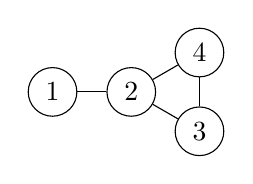
\begin{tikzpicture}
        	\node [circle, draw, align=center] (w1) at (0,0) {$1$};
        	\node [circle, draw, align=center] (w2) at (1,0) {$2$};
        	\node [circle, draw, align=center] (w3) at (1.866,-.5) {$3$};
        	\node [circle, draw, align=center] (w4) at (1.866,.5) {$4$};
	\foreach \from/\to in {
		w1/w2, w2/w3, w2/w4, w3/w4}
	\draw (\from) to (\to);	
	\end{tikzpicture}
	
\

decategorifies like magnitude as shown
\column{.65\textwidth}

\includegraphics[trim = 25mm 70mm 25mm 70mm, clip, keepaspectratio, width=\textwidth]{localGraphics/martiniCategorify2.pdf}
\end{columns}
\end{frame}


\begin{frame}{Categorification helps analyze weighting}

\begin{columns}
\column{.34\textwidth}
Magnitude homology of 

\

	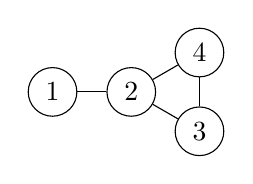
\begin{tikzpicture}
        	\node [circle, draw, align=center] (w1) at (0,0) {$1$};
        	\node [circle, draw, align=center] (w2) at (1,0) {$2$};
        	\node [circle, draw, align=center] (w3) at (1.866,-.5) {$3$};
        	\node [circle, draw, align=center] (w4) at (1.866,.5) {$4$};
	\foreach \from/\to in {
		w1/w2, w2/w3, w2/w4, w3/w4}
	\draw (\from) to (\to);	
	\end{tikzpicture}
	
\

decategorifies like weighting as shown
\column{.65\textwidth}

\includegraphics[trim = 25mm 70mm 25mm 70mm, clip, keepaspectratio, width=\textwidth]{localGraphics/martiniCategorify1.pdf}
\end{columns}
\end{frame}


    %directsum = @(A,B) [A,zeros(size(A,1),size(B,2));zeros(size(B,1),size(A,2)),B];
    %foo = directsum(directsum(ones(5,4),ones(4,3)),ones(3,2));
    %bar = [zeros(size(foo,1),5),foo;zeros(2,size(foo,2)+5)];
    %D = digraph(bar);
    %d = distances(D);
    %t = logspace(-2,1,100);
    %mag = nan(size(t));
    %w = nan(size(d,1),numel(t));
    %for j = 1:numel(t)
    %    Z = exp(-t(j)*d); 
    %    w(:,j) = Z\ones(size(Z,1),1);
    %    mag(j) = sum(Z\ones(size(Z,1),1)); 
    %end
    %% figure; semilogx(t,mag);
    %%%
    %figure('Position',[0,0,280,210]);
    %plo = plot(D,'k');
    %plo.NodeFontSize = 14;
    %plo.LineWidth = 1;
    %plo.Interpreter = 'latex';
    %axis square;
    %daspect([1,1,1]);
    %axis off;
    %fileDir = '/Users/stevehuntsman/Documents/Steve/CatCap/CatCapBeamerTheme/localGraphics';
    %fileName = 'MLP';
    %print([fileDir,filesep,fileName],'-r600','-dpng');
    %print([fileDir,filesep,fileName],'-r600','-dpdf');
    %%%
    %blur = 0;
    %eulerian = 0;
    %K = 8;
    %% L = 0:K;
    %L = 0:(K-1)*max(d(isfinite(d)));
    %%%
    %[allReps,betti,L,allSimplices,allLengths,allMC,allBoundary] = ...
    %    magnitudeHomology(D,K,blur,eulerian,L); 
    %%%
    %coeff = sum(diag((-1).^(0:(K-1)))*betti);
    %foo = coeff*exp(-L'*t);
    %% figure; 
    %% semilogx(t,mag,'k',t,foo,'r.');
    %%%
    %% For 
    %%   D = graph([0,1,2,3]+1,[1,2,3,1]+1);
    %% a little pattern matching strongly suggests that we have betti = diag(b)
    %% where b is given along the lines of the code below
    %K = [1,2,3,4];
    %foo = [];
    %figure;
    %plot(t,mag,'k.-');
    %hold on;
    %for i = 1:numel(K)
    %    a = diag(betti);
    %    b = [a(:)',zeros(1,K(i)-numel(a))]; 
    %    b = b(1:K(i));
    %    coeff = (-1).^(0:(numel(b)-1)).*b(:)';
    %    foo(i,:) = coeff*exp(-(0:numel(b)-1)'*t);
    %    plot(t,foo(i,:),'o-','Color',[numel(K)-i,0,i-1]/(numel(K)-1));
    %end
    %% twoX = 2*strongCutoff(d);
    %% magAtTwoX = sum(exp(-twoX*d)\ones(size(d,1),1)); 
    %% plot(twoX,magAtTwoX,'ko','MarkerSize',10);
    %% plot(log(2)*[1,1],[1,size(D.Nodes,1)],'k:')
    %set(gca,'XScale','log');
    %legend(["magnitude",append("$K=",string(K),"$")],...%,"$2\cdot$cutoff","$\log 2$"],...
    %    'Interpreter','latex','Location','southeast');
    %% ylim([1,size(D.Nodes,1)]);
    %title('partial sums of decategorification','Interpreter','latex');
    %box on;
    %xlabel('$t$','Interpreter','latex');
    %fileName = 'mlpCategorify1';
    %print([fileDir,filesep,fileName],'-r600','-dpng');
    %print([fileDir,filesep,fileName],'-r600','-dpdf');
    %
    %%%
    %cmax = 6;
    %rnk = @(x)(size(x,1)>0)*size(x,2);  % for computing ranks
    %figure('Position',[0,0,560,560]);
    %ha = tight_subplot(size(D.Nodes,1),size(D.Nodes,1),.02,.01,.01);
    %c = 0;
    %for src = 1:size(D.Nodes,1)
    %    for tar = 1:size(D.Nodes,1)
    %        c = c+1;
    %        j = sub2ind([size(D.Nodes,1),size(D.Nodes,1)],tar,src);
    %        axes(ha(j)); %#ok<LAXES> 
    %        b = cellfun(rnk,allReps{src,tar});
    %        b = b(1:4,1:4);
    %        b(b==0) = nan;  % for visibility
    %        pcolor([[b,nan(size(b,1),1)];nan(1,size(b,2)+1)]);
    %        view([0,0,-90]);
    %        axis off;
    %        [foo,ind] = max(b,[],'all');
    %        [i1,i2] = ind2sub(size(b),ind);
    %        if ~isnan(foo)
    %            if foo <= cmax/2
    %                text(i1+.25,i2+.5,num2str(foo),'Color','w','FontSize',8);
    %            else
    %                text(i1+.25,i2+.5,num2str(foo),'FontSize',8);
    %            end
    %        end
    %        clim([0,cmax]);
    %    end
    %end
    %f = gcf;
    %exportgraphics(gcf,'/Users/stevehuntsman/Documents/Steve/CatCap/CatCapBeamerTheme/localGraphics/mlpBetti.png','Resolution',600);
    %exportgraphics(gcf,'/Users/stevehuntsman/Documents/Steve/CatCap/CatCapBeamerTheme/localGraphics/mlpBetti.pdf','Resolution',600);
    %% fileName = 'mlpBetti';
    %% print([fileDir,filesep,fileName],'-r600','-dpng');
    %% print([fileDir,filesep,fileName],'-r600','-dpdf');
    %
    %%%
    %% For a DAG the dimensions of simplices and lengths are bounded and the
    %% categorification formula for magnitude homology becomes possible to
    %% evaluate without analytical computations (at least in principle). Think
    %% in particular of MLPs with quantized weights (for, e.g., low-energy
    %% implementations) as being particularly amenable to this sort of thing.


\begin{frame}{DAGs are very nicely handled}

\begin{columns}
\column{.34\textwidth}
Magnitude homology of \emph{multilayer perceptron} (MLP) $K^\rightarrow_{5,4,3,2}$

\includegraphics[trim = 75mm 115mm 75mm 115mm, clip, keepaspectratio, width=\textwidth]{localGraphics/MLP.pdf}

decategorifies as shown
\column{.65\textwidth}

\includegraphics[trim = 25mm 70mm 25mm 70mm, clip, keepaspectratio, width=\textwidth]{localGraphics/mlpCategorify1.pdf}
\end{columns}
\end{frame}


\begin{frame}{DAGs are very nicely handled}

\begin{columns}
\column{.34\textwidth}
Magnitude homology of \emph{multilayer perceptron} (MLP) $K^\rightarrow_{5,4,3,2}$

\includegraphics[trim = 75mm 115mm 75mm 115mm, clip, keepaspectratio, width=\textwidth]{localGraphics/MLP.pdf}

has Betti numbers shown
\column{.65\textwidth}
\centering
\includegraphics[trim = 0mm 0mm 0mm 0mm, clip, keepaspectratio, width=.8\textwidth]{localGraphics/mlpBetti.pdf}
\end{columns}
\end{frame}

    %%%
    %directsum = @(A,B) [A,zeros(size(A,1),size(B,2));zeros(size(B,1),size(A,2)),B];
    %nn = [10,2,8,4,6];
    %foo = directsum(directsum(directsum(ones(nn(1),nn(2)),ones(nn(2),nn(3))),ones(nn(3),nn(4))),ones(nn(4),nn(5)));
    %bar = [zeros(size(foo,1),nn(1)),foo;zeros(nn(5),size(foo,2)+nn(1))];
    %D = digraph(bar);
    %
    %%%
    %% rng('default');
    %% n = 6;
    %% A = sprand(n,n,1/n);
    %% D = digraph(A>0);
    %% figure; plot(D);
    %% % Expect betti to be [4,0,0,0,0;0,0,3,0,0]...
    %
    %%%
    %% D = digraph([0,1,1;1,0,1;1,0,0]);
    %% figure; plot(D);
    %% % Expect betti to be [5,0,0,0,0,0;0,7,0,0,0,0;0,0,9,0,0,0;0,0,0,11,0,0]...
    %
    %%% If D has no weights, add unit weights; remove any loops and get size
    %% Weights
    %foo = string(D.Edges.Properties.VariableNames);
    %if nnz(foo=="Weight") == 0
    %    D.Edges.Weight = ones(size(D.Edges,1),1);
    %end
    %% Loops
    %D = simplify(D);
    %% Size
    %n = size(D.Nodes,1);
    %
    %%%
    %d = distances(D);
    %% Reachability weighted by distances
    %distanceDigraph = digraph(d);
    %distanceDigraph = ...
    %    rmedge(distanceDigraph,find(isinf(distanceDigraph.Edges.Weight)));
    %Ad = adjacency(distanceDigraph); % NOT weighted
    %
    %%%
    %blur = 0;
    %K = 5;
    %L = 0:6;%(K+1);
    %minLen = 0;
    %maxLen = L(end);
    %maxNum = 1000;
    %
    %%%
    %aggregateBetti = zeros(K,numel(L));
    %betti = cell(n,n);
    %for s = 1:n
    %    for t = 1:n
    %        [s,t]
    %        %% Simplices and their lengths
    %        % Nondegenerate simplices are paths from s to t in distanceDigraph
    %        simplices = cell(1,K+1);
    %        lengths = cell(1,K+1);
    %%         % k = 0 nonempty iff s = t
    %%         if s == t
    %%             simplices{0+1} = s;
    %%             lengths{0+1} = 0;
    %%         end
    %        % Compute number of paths from s to t in distanceDigraph that have
    %        % hop lengths from 0 to K, i.e., the number of simplices
    %        pow = eye(size(Ad));
    %        num = zeros(1,K+1);
    %        for k = 0:K
    %            num(k+1) = pow(s,t);
    %            if k < K
    %                pow = pow*Ad;
    %            end
    %        end
    %        % Get the paths, then filter simplices by hop grading and get
    %        % lengths (this is reasonably efficient but still far from
    %        % optimal). It's not clear how to effi
    %        if sum(num) > 0
    %            % NB. Using allpaths and allcycles would be tricky and
    %            % burdensome. Fortunately we can freely use
    %            % https://github.com/SteveHuntsmanBAESystems/BasicPathHomology/blob/master/reashortestpaths.m
    %            paths = reashortestpaths(distanceDigraph,s,t,sum(num));
    %            hops = cellfun(@numel,paths)-1;
    %            for k = 0:K
    %                simplices{k+1} = cell2mat(paths(hops==k)');
    %                lengths{k+1} = zeros(size(simplices{k+1},1),1);
    %                for j = 1:size(simplices{k+1},1)
    %                    for i = 1:(size(simplices{k+1},2)-1)
    %                        lengths{k+1}(j) = lengths{k+1}(j)...
    %                            +d(simplices{k+1}(j,i),simplices{k+1}(j,i+1));
    %                    end
    %                end
    %            end
    %        end
    %
    %        %% Relation to be applied on lengths and grading
    %        % Use numerically well-behaved equality predicate to avoid any
    %        % floating point badness that might have been inherited in D
    %        if blur % blurred magnitude homology
    %            rel = @(x1,x2) le(x1,x2);   % x1 <= x2
    %        else    % vanilla magnitude homology
    %            rel = @(x1,x2) eq(x1,x2);   % x1 == x2
    %%             % Use a loosening of rel = @(x1,x2) eq(x1,x2) for floats
    %%             rel = @(x1,x2) (max(x1-x2)-min(x1,x2)) < sqrt(eps)*mean(x1,x2);
    %%             rel = @(x1,x2) 1-min(x1,x2)/max(x1,x2) < sqrt(eps);
    %        end
    %        
    %        %% Chains
    %        MC = cell(K+1,numel(L));
    %        for ell = 1:numel(L)
    %            if L(ell) == 0
    %                MC{0+1,ell} = simplices{0+1};
    %            end
    %            for k = 0:K
    %                MC{k+1,ell} = simplices{k+1}(rel(lengths{k+1},L(ell)),:);
    %            end
    %        end
    %        
    %        %% Boundary matrices
    %        boundary = cell(K,numel(L));
    %        for k = 1:K
    %            for ell = 1:numel(L)
    %                boundaryInit = ...
    %                    sparse(size(MC{k-1+1,ell},1),size(MC{k+1,ell},1));
    %                boundary{k+1,ell} = boundaryInit;
    %                %
    %                for j = 1:(k-1)
    %                    boundary_j = boundaryInit;
    %                    for i = 1:size(MC{k+1,ell},1)
    %                        neg = MC{k+1,ell}(i,j+1-1);
    %                        nil = MC{k+1,ell}(i,j+1);
    %                        pos = MC{k+1,ell}(i,j+1+1);
    %                        if rel(d(neg,pos),d(neg,nil)+d(nil,pos))
    %                            del = MC{k+1,ell}(i,setdiff(0:k,j)+1);
    %                            ind = ismember(MC{k-1+1,ell},del,'rows','legacy');
    %                            boundary_j(ind,i) = 1; %#ok<SPRIX> 
    %                        end
    %                    end
    %                    boundary{k+1,ell} = boundary{k+1,ell}+((-1)^j)*boundary_j;
    %                end
    %            end
    %        end
    %
    %        %%
    %%         [KK,LL] = find(~cellfun(@isempty,MC));
    %%         for jj = 1:numel(KK)
    %%             stkl0 = [s,t;KK(jj)-1,LL(jj)-1]
    %%             mc = MC{KK(jj),LL(jj)}
    %%             bdry = boundary{KK(jj),LL(jj)}
    %%         end
    %
    %        %% Dimensions of boundary map images and kernels
    %        dimIm = zeros(K+1,numel(L));
    %        dimKer = zeros(K+1,numel(L));
    %        for k = 0:K
    %            for ell = 1:numel(L)
    %                bdry = boundary{k+1,ell};
    %                dimIm(k+1,ell) = rank(full(bdry(any(bdry,2),:))); % kill zero columns
    %                % dimIm(k+1,ell) = rank(sym(bdry(any(bdry,2),:)));
    %                if size(bdry,2)%~isempty(bdry)
    %                    dimKer(k+1,ell) = size(bdry,2)-dimIm(k+1,ell);  
    %                end
    %            end
    %        end
    %        
    %        %% Betti numbers
    %        betti{s,t} = dimKer((0:(K-1))+1,:)-dimIm((1:K)+1,:);
    %%         bettist = betti{s,t}
    %        aggregateBetti = aggregateBetti+betti{s,t};
    %    end
    %end
    %aggregateBetti
    %
    %%%
    %% figure;
    %% c = 0;
    %% for s = 1:n
    %%     for t = 1:n
    %%         c = c+1;
    %%         subplot(n,n,c);
    %%         b = betti{s,t};
    %%         b(b==0) = nan;  % for visibility
    %%         pcolor([[b,nan(size(b,1),1)];nan(1,size(b,2)+1)]);
    %%         axis off;
    %%         foo = cellfun(@max,betti,'UniformOutput',false);
    %%         bar = cellfun(@max,foo,'UniformOutput',false);
    %%         clim([0,max(cell2mat(bar),[],'all')]);
    %%         if s == 1 && t == 1
    %%             title(['max(clim) = ',num2str(max(cell2mat(bar),[],'all'))]);
    %%         end
    %%     end
    %% end
    %
    %%%
    %% foo = [];
    %% for k = 1:K
    %%     for ell = 1:numel(L)
    %%         foo{k,ell} = [];
    %%         for s = 1:n
    %%             for t = 1:n
    %%                 bar = MCst{s,t}{k,ell};
    %%                 foo{k,ell} = [foo{k,ell},zeros(size(foo{k,ell},1),size(bar,2));...
    %%                     zeros(size(bar,1),size(foo{k,ell},2)),bar];
    %%             end
    %%         end
    %%     end
    %% end

\begin{frame}{Fully connected MLPs have simple MH}

\begin{itemize}
	\item Let $N_\ell := \sum_{i = 1}^{\ell} n_i$, $e_{(\ell)} := \sum_{j=N_{\ell-1}+1}^{N_\ell} e_j$, and $B[x_1,\dots,x_{L-k};n] := \sum_{\ell=1}^{L-k} x_\ell e_{(\ell)}^T e_{(\ell+k)}$
	\begin{itemize}
		\item E.g. $A = B[1_1,\dots,1_{L-1};n]$
	\end{itemize}
\end{itemize}

\begin{alertblock}{The preceding slide's mechanics suggest the conjecture (exercise)}
For $k > 1$, $\beta_{k+1,m}^{(s,t)}(K^\rightarrow_{n_1,\dots,n_L}) = \delta_{k+1,m} \cdot \left ( B \left [ \prod_{\ell = 2}^{k+1} (n_\ell-1), \dots, \prod_{\ell = L-k}^{L-1} (n_\ell-1) ; n \right ] \right )_{st}$ 
\end{alertblock}

Note that we automatically have $\beta_{0,m}^{(s,t)} = \delta_{0m} \delta_{st}$ and $\beta_{1,m}^{(s,t)} = \delta_{1m} A_{st}$

\begin{block}{Examples:}
$\beta(K^\rightarrow_{5,4,3,2}) = \text{diag}(14,38,61,60,0,0,\dots)$ \\
$\beta(K^\rightarrow_{2,11,3,7,5}) = \text{diag}(28,111,304,940,1200,0,0,\dots)$ \\
$\beta(K^\rightarrow_{10,2,8,4,6}) = \text{diag}(30,92,280,532,1260,0,0,\dots)$
\end{block}
\end{frame}


\begin{frame}{Sparsely connected MLPs are more relevant}

\begin{block}{Sparsity arises via (e.g.) pruning small edge weights in trained networks}
``Lottery tickets'' exhibit hierarchical modularity [Patil, Michael, and Dovrolis]
\end{block}

\begin{alertblock}{Magnitude homology might usefully indicate structure\dots}
\dots insofar as it manifests as ``convexity defects'' that differ from a null model
\end{alertblock}

\begin{block}{We provide some \emph{very preliminary} supporting evidence}
Sparse interconnections of MLPs and sparsification of a single MLP both induce off-diagonal magnitude homology, but differently
\end{block}
\end{frame}


    %%%
    %directsum = @(A,B) [A,zeros(size(A,1),size(B,2));zeros(size(B,1),size(A,2)),B];
    %nn = [8,4,4,4,2];
    %% nn = [12,6,6,6,3];
    %% nn = [16,8,8,8,4];
    %foo = directsum(ones(nn(1),nn(2)),ones(nn(2),nn(3)));
    %for j = 2:(numel(nn)-1)
    %    foo = directsum(foo,ones(nn(j),nn(j+1)));
    %end
    %bar = [zeros(size(foo,1),nn(1)),foo;zeros(nn(end),size(foo,2)+nn(1))];
    %%
    %foo0 = directsum(ones(nn(1),nn(2)),zeros(nn(2),nn(3)));
    %for j = 2:(numel(nn)-1)
    %    if j < numel(nn)-1
    %        foo0 = directsum(foo0,zeros(nn(j),nn(j+1)));
    %    else
    %        foo0 = directsum(foo0,ones(nn(j),nn(j+1)));
    %    end
    %end
    %bar0 = [zeros(size(foo0,1),nn(1)),foo0;zeros(nn(end),size(foo0,2)+nn(1))];
    %%
    %rng('default');
    %threshInternal = 1;
    %threshExternal = 1/8;
    %twoCol = [bar.*(rand(size(bar))<threshInternal),...
    %    bar0.*(rand(size(bar0))<threshExternal);...
    %    bar0.*(rand(size(bar0))<threshExternal),...
    %    bar.*(rand(size(bar))<threshInternal)];
    %D = digraph(twoCol);
    %
    %%% If D has no weights, add unit weights; remove any loops and get size
    %% Weights
    %foo = string(D.Edges.Properties.VariableNames);
    %if nnz(foo=="Weight") == 0
    %    D.Edges.Weight = ones(size(D.Edges,1),1);
    %end
    %% Loops
    %D = simplify(D);
    %% Size
    %n = size(D.Nodes,1);
    %
    %%%
    %% figure; plot(D,'Layout','layered');
    %
    %%%
    %K = 6;
    %blur = 0;
    %eulerian = 0;
    %L = 0:(K+1);%(K-1);
    %
    %%%
    %[allReps,betti,L,allSimplices,allLengths,allMC,allBoundary] = ...
    %    magnitudeHomology(D,K,blur,eulerian,L); 
    %
    %%%
    %betti
    %
    %%%
    %figure; 
    %plo = plot(D,'NodeColor','k','EdgeColor','k','NodeLabel',[],'Layout','layered');
    %% Clean up layers (hacky)
    %for j = 1:size(D.Nodes,1)
    %    succ = successors(D,j);
    %    if ~isempty(succ)
    %        if any(plo.YData(succ)) ~= plo.YData(j)-1
    %            plo.YData(j) = min(plo.YData(succ))+1;
    %        end
    %    end
    %end
    %axis off;
    %
    %%% Get largest weak component of D
    %wc = conncomp(D,'Type','weak');
    %foo = histcounts(wc);
    %[~,largestWC] = max(foo);
    %indLargestWC = find(wc==largestWC);
    %D_weak = subgraph(D,indLargestWC);
    %
    %%% Undirected version
    %UD_weak = graph(max(adjacency(D_weak),adjacency(D_weak).'));
    %
    %%% Spectral bipartition of undirected version of D_weak
    %% https://www.mathworks.com/help/matlab/math/partition-graph-with-laplacian-matrix.html
    %lap = laplacian(UD_weak);
    %[vec,diag] = eigs(lap,2,'smallestabs');
    %fiedlerVector = vec(:,2);
    %highlight(plo,indLargestWC(fiedlerVector>=0),'NodeColor','r'); % subgraph A
    %highlight(plo,indLargestWC(fiedlerVector<0),'NodeColor','b'); % subgraph B
    %% Indices of cut edges in D_weak
    %cutInd_weak = find(prod(fiedlerVector(UD_weak.Edges.EndNodes),2)<0);
    %% Cut edges in D_weak
    %foo = UD_weak.Edges(cutInd_weak,:).EndNodes;
    %undirectedCutEdges = [foo;fliplr(foo)];
    %% Cut edges in D
    %cutInd = ...
    %    find(ismember(D.Edges.EndNodes,indLargestWC(undirectedCutEdges),'rows'));
    %directedCutEdges = D.Edges.EndNodes(cutInd,:);
    %highlight(plo,directedCutEdges(:,1),directedCutEdges(:,2),...
    %    'EdgeColor',[.5,0,.5]);%,'LineStyle','--');
    %
    %%% Collect off-diagonal contributions to Betti numbers
    %offDiagBettiContribs = zeros(size(adjacency(D)));
    %for k = 0:(K-1)
    %    for ell = 1:numel(L)
    %        if k ~= L(ell)
    %            foo = @(x) numel(x{k+1,ell});
    %            offDiagBettiContribs = offDiagBettiContribs+cellfun(foo,allReps);
    %        end
    %    end
    %end
    %
    %%%
    %ODBC = digraph(offDiagBettiContribs);
    %hold on;
    %plo = plot(ODBC,'XData',plo.XData,'YData',plo.YData,'EdgeColor',[225,175,64]/255,...%'k',...
    %    'LineStyle',':','ArrowSize',0,'NodeLabel',[],'LineWidth',2);
    %highlight(plo,find(fiedlerVector>=0),'NodeColor','r') % subgraph A
    %highlight(plo,find(fiedlerVector<0),'NodeColor','b') % subgraph B
    %
    %%%
    %fileDir = '/Users/stevehuntsman/Documents/Steve/CatCap/CatCapBeamerTheme/localGraphics';
    %fileName = 'MLPx2';
    %print([fileDir,filesep,fileName],'-r600','-dpng');
    %print([fileDir,filesep,fileName],'-r600','-dpdf');

\begin{frame}{Sparse interconnections $\Rightarrow$ off-diagonals}

\begin{columns}
\column{.49\textwidth}
$$\beta = \begin{pmatrix}
 52 & 0 & 0 & 0 & 0 & 0 & 0 & \dots \\
 0 & 182 & 0 & 0 & 0 & 0 & 0 & \dots \\
 0 & 0 & 436 & 0 & 0 & {\color{CatCapGold}4} & 0 & \dots \\
 0 & 0 & 0 & 1020 & 0 & 0 & 0 & \dots \\
 0 & 0 & 0 & 0 & 2196 & 0 & 0 & \dots \\
 0 & 0 & 0 & 0 & 0 & 2646 & 0 & \dots \\
 0 & 0 & 0 & 0 & 0 & 0 & 0 & \dots \\
 \vdots & \vdots & \vdots & \vdots & \vdots & \vdots & \vdots & \ddots
\end{pmatrix}$$

Off-diagonal contributions indicated by {\color{CatCapGold}dotted lines from sources to targets}

\

{\color{red}Vertices} {\color{blue}colored} by undirected Fiedler vector (i.e., spectral) bipartition; {\color{violet}traversing arcs are purple}

\column{.49\textwidth}
\includegraphics[trim = 45mm 90mm 45mm 90mm, clip, keepaspectratio, width=\textwidth]{localGraphics/MLPx2.pdf}
\end{columns}
\end{frame}


    %%%
    %directsum = @(A,B) [A,zeros(size(A,1),size(B,2));zeros(size(B,1),size(A,2)),B];
    %% nn = [8,4,4,4,2];
    %% nn = [12,6,6,6,3];
    %nn = [16,8,8,8,4];
    %foo = directsum(ones(nn(1),nn(2)),ones(nn(2),nn(3)));
    %for j = 2:(numel(nn)-1)
    %    foo = directsum(foo,ones(nn(j),nn(j+1)));
    %end
    %bar = [zeros(size(foo,1),nn(1)),foo;zeros(nn(end),size(foo,2)+nn(1))];
    %D = digraph(bar.*(rand(size(bar))<2/5));
    %% %
    %% foo0 = directsum(ones(nn(1),nn(2)),zeros(nn(2),nn(3)));
    %% for j = 2:(numel(nn)-1)
    %%     if j < numel(nn)-1
    %%         foo0 = directsum(foo0,zeros(nn(j),nn(j+1)));
    %%     else
    %%         foo0 = directsum(foo0,ones(nn(j),nn(j+1)));
    %%     end
    %% end
    %% bar0 = [zeros(size(foo0,1),nn(1)),foo0;zeros(nn(end),size(foo0,2)+nn(1))];
    %% %
    %% rng('default');
    %% threshInternal = 1;
    %% threshExternal = 1/8;
    %% twoCol = [bar.*(rand(size(bar))<threshInternal),...
    %%     bar0.*(rand(size(bar0))<threshExternal);...
    %%     bar0.*(rand(size(bar0))<threshExternal),...
    %%     bar.*(rand(size(bar))<threshInternal)];
    %% D = digraph(twoCol);
    %
    %%% If D has no weights, add unit weights; remove any loops and get size
    %% Weights
    %foo = string(D.Edges.Properties.VariableNames);
    %if nnz(foo=="Weight") == 0
    %    D.Edges.Weight = ones(size(D.Edges,1),1);
    %end
    %% Loops
    %D = simplify(D);
    %% Size
    %n = size(D.Nodes,1);
    %
    %%%
    %% figure; plot(D,'Layout','layered');
    %
    %%%
    %K = 6;
    %blur = 0;
    %eulerian = 0;
    %L = 0:(K+1);%(K-1);
    %
    %%%
    %[allReps,betti,L,allSimplices,allLengths,allMC,allBoundary] = ...
    %    magnitudeHomology(D,K,blur,eulerian,L); 
    %
    %%%
    %betti
    %
    %%%
    %figure; 
    %plo = plot(D,'NodeColor','k','EdgeColor','k','NodeLabel',[],'Layout','layered');
    %% Clean up layers (hacky)
    %for j = 1:size(D.Nodes,1)
    %    succ = successors(D,j);
    %    if ~isempty(succ)
    %        if any(plo.YData(succ)) ~= plo.YData(j)-1
    %            plo.YData(j) = min(plo.YData(succ))+1;
    %        end
    %    end
    %end
    %axis off;
    %
    %% %% Get largest weak component of D
    %% wc = conncomp(D,'Type','weak');
    %% foo = histcounts(wc);
    %% [~,largestWC] = max(foo);
    %% indLargestWC = find(wc==largestWC);
    %% D_weak = subgraph(D,indLargestWC);
    %% 
    %% %% Undirected version
    %% UD_weak = graph(max(adjacency(D_weak),adjacency(D_weak).'));
    %% 
    %% %% Spectral bipartition of undirected version of D_weak
    %% % https://www.mathworks.com/help/matlab/math/partition-graph-with-laplacian-matrix.html
    %% lap = laplacian(UD_weak);
    %% [vec,diag] = eigs(lap,2,'smallestabs');
    %% fiedlerVector = vec(:,2);
    %% highlight(plo,indLargestWC(fiedlerVector>=0),'NodeColor','r'); % subgraph A
    %% highlight(plo,indLargestWC(fiedlerVector<0),'NodeColor','b'); % subgraph B
    %% % Indices of cut edges in D_weak
    %% cutInd_weak = find(prod(fiedlerVector(UD_weak.Edges.EndNodes),2)<0);
    %% % Cut edges in D_weak
    %% foo = UD_weak.Edges(cutInd_weak,:).EndNodes;
    %% undirectedCutEdges = [foo;fliplr(foo)];
    %% % Cut edges in D
    %% cutInd = ...
    %%     find(ismember(D.Edges.EndNodes,indLargestWC(undirectedCutEdges),'rows'));
    %% directedCutEdges = D.Edges.EndNodes(cutInd,:);
    %% highlight(plo,directedCutEdges(:,1),directedCutEdges(:,2),...
    %%     'EdgeColor',[.5,0,.5]);%,'LineStyle','--');
    %
    %%% Collect off-diagonal contributions to Betti numbers
    %offDiagBettiContribs = zeros(size(adjacency(D)));
    %for k = 0:(K-1)
    %    for ell = 1:numel(L)
    %        if k ~= L(ell)
    %            foo = @(x) numel(x{k+1,ell});
    %            offDiagBettiContribs = offDiagBettiContribs+cellfun(foo,allReps);
    %        end
    %    end
    %end
    %
    %%%
    %ODBC = digraph(offDiagBettiContribs);
    %hold on;
    %plo = plot(ODBC,'XData',plo.XData,'YData',plo.YData,'EdgeColor',[225,175,64]/255,...%'k',...
    %    'LineStyle',':','ArrowSize',0,'NodeLabel',[],'LineWidth',2,'NodeColor','k');
    %% highlight(plo,find(fiedlerVector>=0),'NodeColor','r') % subgraph A
    %% highlight(plo,find(fiedlerVector<0),'NodeColor','b') % subgraph B
    %
    %%%
    %fileDir = '/Users/stevehuntsman/Documents/Steve/CatCap/CatCapBeamerTheme/localGraphics';
    %fileName = 'MLPsparsified';
    %print([fileDir,filesep,fileName],'-r600','-dpng');
    %print([fileDir,filesep,fileName],'-r600','-dpdf');

\begin{frame}{Sparsification $\Rightarrow$ off-diagonals (differently)}

\begin{columns}
\column{.49\textwidth}
$$\beta = \begin{pmatrix}
52 & 0 & 0 & 0 & 0 & 0 & 0 & \dots \\
0 & 143 & 0 & 0 & 0 & 0 & 0 & \dots \\
0 & 0 & 164 & {\color{CatCapGold}44} & {\color{CatCapGold}5} & 0 & 0 & \dots \\
0 & 0 & 0 & 71 & {\color{CatCapGold}71} & {\color{CatCapGold}38} & 0 & \dots \\
0 & 0 & 0 & 0 & 2 & {\color{CatCapGold}47} & 0 & \dots \\
0 & 0 & 0 & 0 & 0 & 0 & 0 & \dots \\
 \vdots & \vdots & \vdots & \vdots & \vdots & \vdots & \vdots & \ddots
\end{pmatrix}$$

Off-diagonal contributions indicated by {\color{CatCapGold}dotted lines from sources to targets}

\

Keeping $\approx 2/5$ of arcs in $K^\rightarrow_{16,8,8,8,8,4}$

\column{.49\textwidth}
\includegraphics[trim = 45mm 90mm 45mm 90mm, clip, keepaspectratio, width=\textwidth]{localGraphics/MLPsparsified.pdf}
\end{columns}
\end{frame}


\begin{frame}{This may be useful in practice}

\begin{block}{Deep neural networks are functionally sparsified and modular}
Weight filtrations (for sparsity) and quantizations (for efficiency) are common
\end{block}

%\begin{block}{A ``null model'' of IID arc weights may actually be fairly realistic}
%Neural networks are initialized randomly; training finds one of many extrema
%\end{block}

\begin{block}{For a DAG the dimensions of simplices and lengths are bounded} 
In this case numerics largely suffice: e.g. the (de)categorification formula 
$$((\exp[-\tau d])^{-1})_{st} \overset{\tau \gg 0}{=} \sum_{k,L} (-1)^k \text{rank} \left ( MH_{k,L}^{(s,t)} \right ) \exp(-\tau L) = \sum_L \chi_{\bullet,L}^{(s,t)} \exp(-\tau L)$$ 
can exactly produce $\chi_{\bullet,L}^{(s,t)}$ via Laplace transform \emph{without ever computing} $MH$
\end{block}

\begin{alertblock}{}
\end{alertblock}

\end{frame}


\begin{frame}{Consider a whole-animal connectome}

\begin{columns}
\column{.33\textwidth}
Whole-animal chemical connectome of hermaphroditic \emph{Caenorhabditis elegans} (nematode) is a digraph with 454 vertices and 4879 arcs (see \url{https://wormwiring.org})

\

{\color{CatCapGold}The pharynx subconnectome with 50 vertices and 242 arcs is in the box at upper left}

\column{.66\textwidth}
\includegraphics[trim = 50mm 95mm 45mm 85mm, clip, keepaspectratio, width=\textwidth]{localGraphics/GHermChem.pdf}
\end{columns}
\end{frame}


    %%%
    %% Digraph from https://www.wormwiring.org/pages/software.html
    %file = '/Users/stevehuntsman/Downloads/wormwiring/GHermChem.mat';
    %% file = '/Users/stevehuntsman/Downloads/wormwiring/GMaleChem.mat';
    %load(file);
    %%     {'BodyWallMuscles' }
    %%     {'InterNeurons'    }
    %%     {'MotorNeurons'    }
    %%     {'OtherEndOrgans'  }
    %%     {'Pharynx'         }
    %%     {'SensoryNeurons'  }
    %%     {'SexSpecificCells'}
    %% D = GHermChem;
    %D = subgraph(GHermChem,...
    %    find(matches(GHermChem.Nodes.Group,["Pharynx"])));
    %D.Edges.Weight = ones(size(D.Edges.Weight));
    %D = simplify(D);
    %
    %%%
    %d = distances(D,'Method','unweighted');
    %
    %%% Determine betweenness, adjacency, and Menger convexity
    %between = cell(size(d));
    %strictlyBetween = cell(size(d));
    %for x = 1:size(d,1)
    %    for z = 1:size(d,2)
    %        between{x,z} = find(d(x,:)+d(:,z)'==d(x,z));
    %        strictlyBetween{x,z} = setdiff(between{x,z},[x,z]);
    %    end
    %end
    %%
    %adjacent = cellfun(@isempty,strictlyBetween);
    %diagonal = diag(true(size(d,1),1));
    %MengerConvex = ~any(~diagonal&adjacent,'all');
    %
    %%% Determine unique non-adjacency and geodeticness
    %uniquelyNonAdjacent = true(size(d));
    %for x = 1:size(d,1)
    %    for z = 1:size(d,2)
    %        for i1 = 1:numel(between{x,z})
    %            for i2 = 1:numel(between{x,z})
    %                y1 = between{x,z}(i1);
    %                y2 = between{x,z}(i2);
    %                foo = ismember(y1,between{x,y2})&ismember(y2,between{y1,z});
    %                bar = ismember(y2,between{x,y1})&ismember(y1,between{y2,z});
    %                if foo||bar == false
    %                    uniquelyNonAdjacent(x,z) = false;
    %                    continue;
    %                end
    %            end
    %        end
    %    end
    %end
    %%
    %geodetic = ~any(~diagonal&~uniquelyNonAdjacent,'all');
    %
    %%% Determine 4-cuts
    %no4Cut = false(size(d));
    %for y1 = 1:size(d,1)
    %    for y2 = 1:size(d,2)
    %        if y1 ~= y2
    %            for x = 1:size(d,1)
    %                for z = 1:size(d,2)
    %                    if d(x,y1)+d(y1,y2)==d(x,y2)&&d(y1,y2)+d(y2,z)==d(y1,z)
    %                        if d(x,z)~=d(x,y1)+d(y1,y2)+d(y2,z)
    %                            no4Cut(x,z) = true;
    %                            continue;
    %                        end
    %                    end
    %                end
    %            end
    %        end
    %    end
    %end
    %figure; spy(no4Cut)
    %noFourCuts = ~diagonal&no4Cut
    %
    %%%
    %blur = 0;
    %eulerian = 0;
    %K = 3;
    %L = 0:(K-1)*max(d(isfinite(d)));
    %
    %%%
    %[allReps,betti,L,allSimplices,allLengths,allMC,allBoundary] = ...
    %    magnitudeHomology(D,K,blur,eulerian,L); 
    %
    %%%
    %save('workspace20230524');
    %
    %%%
    %% betti(3,4) = 11
    %foo = cellfun(@(aR)numel(aR{3,4}),allReps);
    %[src,tar] = find(foo);
    %for j = 1:numel(src)
    %    srctar = [src(j),tar(j)]
    %    [allReps{src(j),tar(j)}{3,4},allMC{src(j),tar(j)}{3,4}]
    %end
    %
    %%%
    %k = 2;
    %ell = 4;
    %figure;
    %ha = tight_subplot(3,4,.01,.01,.01);
    %for j = 1:numel(ha)
    %    %%
    %    axes(ha(j));
    %    if j <= numel(src)
    %        %%
    %        x = allReps{src(j),tar(j)}{k+1,ell};
    %        nzx = find(x~=0);
    %        x = x(nzx);
    %        % Quantize (cf. quantumpcolor)
    %        [ux,~,iu] = uniquetol(x,sqrt(eps));  % x(:) ~ ux(iu)
    %        if numel(ux) > sqrt(numel(x))
    %           warning('numel(uniquetol(x)) > sqrt(numel(x))');
    %        end
    %        ind = reshape(iu,size(x));
    %        % Get quantized colorbar labels (cf. quantumpcolor)
    %        ratError = max(abs(str2num(rats(ux))./(ux+(ux==0))-(ux~=0))); %#ok<ST2NM> 
    %        if ratError < sqrt(eps)
    %           lab = strtrim(string(rats(ux)));
    %        else
    %           lab = string(ux);
    %        end
    %        %
    %        lin_r = linspace(1,0,numel(ux))';
    %        lin_g = zeros(size(lin_r));
    %        lin_b = linspace(0,1,numel(ux))';
    %        cmap = [lin_r,lin_g,lin_b]; % parula(numel(ux));
    %        %
    %        rep = allMC{src(j),tar(j)}{k+1,ell}(nzx,:);
    %        %%
    %        plo = plot(D,'Layout','layered','NodeColor','k','EdgeColor','k',...
    %            'NodeLabel',{},'ArrowSize',0,'MarkerSize',1);
    %        for i = 1:size(rep,1)
    %            [~,~,edgepath0] = shortestpath(D,rep(i,1),rep(i,2));
    %            [~,~,edgepath1] = shortestpath(D,rep(i,2),rep(i,3));
    %            highlight(plo,'Edges',edgepath0,'EdgeColor',cmap(iu(i),:),'LineWidth',3);
    %            highlight(plo,'Edges',edgepath1,'EdgeColor',cmap(iu(i),:),'LineWidth',3);
    %        end
    %        %
    %        ind0 = findnode(D,src(j));
    %        ind1 = findnode(D,tar(j));
    %        str0 = D.Nodes.Name{ind0};
    %        str1 = D.Nodes.Name{ind1};
    %        text(plo.XData(ind0),plo.YData(ind0),str0);
    %        text(plo.XData(ind1),plo.YData(ind1),str1);
    %        % (cf. quantumpcolor)
    %        if numel(lab) > 2
    %            tick = linspace(1.5,numel(lab)-.5,numel(lab));
    %        elseif numel(lab) == 2
    %            tick = linspace(1,numel(lab)-.5,numel(lab));
    %        else
    %            tick = ux;
    %        end
    %        colorbar('Ticks',tick,'TickLabels',lab);%,'Limits',[0,numel(lab)]);
    %        colormap(cmap);
    %        if numel(lab) > 1
    %            clim([1,numel(lab)]);
    %        else
    %            clim(numel(lab)+[-1,1]);
    %        end
    %    end
    %    axis off;
    %end
    %
    %%%
    %k = 3; ell = 6; for src = 1:size(D.Nodes,1), for tar = 1:size(D.Nodes,1), foo = allReps{src,tar}; if ~isempty(foo{k,ell}), [allReps{src,tar}{k,ell},nan(size(allReps{src,tar}{k,ell},1),1),allMC{src,tar}{k,ell}], end, end, end


\begin{frame}{The pharynx has off-diagonal 2-homology}

\begin{columns}
\column{.49\textwidth}
$$\beta = \begin{pmatrix}
50 & 0 & 0 & 0 & 0 & 0 & 0 & 0 & \dots \\
0 & 241 & 0 & 0 & 0 & 0 & 0 & 0 & \dots \\
0 & 0 & 1290 & {\color{CatCapGold}11} & 0 & {\color{CatCapGold}9} & {\color{CatCapGold}13} & 0 & \dots \\
\vdots & \vdots & \vdots & \vdots & \vdots & \vdots & \vdots & \vdots & \ddots
\end{pmatrix}$$

\begin{block}{Off-diagonal 2-homology is intricate}
The subconnectome is not Menger convex or geodetic; it has 4-cuts
\end{block}

\begin{alertblock}{Exercise: $\exists$ biological significance?}
E.g., 10/11 reps for $(k,L) = (2,3)$ either have source neurons M2R, M3R, or NSML, or have target neuron MCR
\end{alertblock}


\column{.49\textwidth}
\includegraphics[trim = 50mm 90mm 40mm 85mm, clip, keepaspectratio, width=\textwidth]{localGraphics/Pharynx.pdf}
\end{columns}
\end{frame}




\begin{frame}{Takeaways}
	\begin{alertblock}<1-> {Magnitude homology might be considered too abstract for real applications}
		But this would be a mistake
	\end{alertblock} 
	\begin{block}<2-> {Magnitude homology is amenable to computation \emph{in silico}}
		It can enable new capabilities for fundamentally discrete data and problems that are ubiquitous in network science, machine learning, and cybersecurity
	\end{block} 
\end{frame}

\framecard{Thanks \\ \ \\ {\large MATLAB code at \url{https://github.com/SteveHuntsman/MagnitudeHomology}}}


%%\section{Before you start}
%\begin{frame}{Overleaf users}
%
%\begin{alertblock}{Warning}
%You can ignore this slide if you're \textbf{not} working with Overleaf.
%\end{alertblock}
%
%\vskip 0.5cm
%
%Overleaf, Beamer and Biber do not always get along well together. For this reason, if you make a mistake while writing this presentation, in the drop-down error message you'll \textbf{always} get Biber-related error messages.
%
%\vskip 0.5cm
%
%Luckily, you just have to click on ``\texttt{go to first error/warning}'' and the UI will scroll to the line containing your mistake.
%
%\end{frame}
%
%\begin{frame}[fragile]
%\frametitle{Compiling}
%
%\begin{alertblock}{Warning}
%You can ignore this slide if you \textbf{are} working with Overleaf.
%\end{alertblock}
%
%To compile this deck you'll need the \texttt{biber} package. Probably your \TeX editor already supports it; if not, you will easily find online the instructions to install it.
%
%\vskip 0.5cm
%
%If you're not using an editor, you can compile this presentation using the command line by running:
%
%\begin{verbatim}
%$ pdflatex main.tex
%$ biber main.bcf
%$ pdflatex main.tex
%$ pdflatex main.tex
%\end{verbatim}
%
%
%\end{frame}
%
%%\section{Colors}
%
%\begin{frame}{Colors}
%
%For this template we defined three colors:
%\begin{itemize}
%\item \textcolor{white}{\marker[CatCapBlue]{\texttt{CatCapBlue}}}
%\item \textcolor{white}{\marker[CatCapGold]{\texttt{CatCapGold}}}
%\item \textcolor{white}{\marker[CatCapSilver]{\texttt{CatCapSilver}}}
%\end{itemize}
%
%\vskip 0.5cm
%
%You can use these colors as you want in your presentation. For example, you can \textbf{\textcolor{CatCapGold}{color the text in Gold}} by writing \texttt{\textbackslash textcolor\{CatCapGold\}\{my green text\}}.
%
%\vskip 0.5cm
%
%We also redefined many of the most common \LaTeX{} and Beamer commands, like \texttt{itemize}, \texttt{block}, etc. You will see samples of these commands in the following slides.
%
%\end{frame}
%
%%\section{Blocks}
%
%\begin{frame} 
%\frametitle{This is a page with a title and a subtitle} 
%\framesubtitle{And also some blocks.} 
%\begin{block}{Goal of the mission}
%Shoot in the Death Star's exhaust port and destroy it before it can fire on the Rebel base.
%\end{block} 
%\begin{alertblock}{Take care!}
%TIE Fighters may chase you while approaching the target.
%\end{alertblock} 
%\begin{exampleblock}{Use the force you must}
%Remember your training with Obi-Wan, and use the Force to make the perfect shot.
%\end{exampleblock} 
%
%\end{frame}
%
%%\section{Enumerates, itemizes and description}
%
%%\subsection{Enumerates and itemizes}
%
%
%\begin{frame}{Enumerates and itemizes}
%
%This is an example of \texttt{itemize}.
%\begin{itemize}
%	\item A long time ago in a galaxy far, far away...
%\end{itemize}
%And this is an example of \texttt{enumerate}.
%
%\begin{enumerate} 
%  \item Go to the Death Star.
%  \item Find the exhaust port.
%  \item Make the perfect shot.
%  \item Become a hero.
%\end{enumerate}
%\end{frame}
%
%%\subsection{Description}
%
%\begin{frame}[fragile]
%\frametitle{Description}
%This is an example of \texttt{description}.
%
%\begin{description}
%\item<2->[Vader] \emph{I am} your father.
%\item<1->[Luke] No. No! That's not true! \textbf{That's impossible!}
%\end{description}
%
%\begin{uncoverenv}<3>
%  \vskip 0.5cm
%  And while we're here, let's have a look to \texttt{verbatim} as well, to see how we made items appear in arbitrary order:
%  \vskip 0.5cm
%  \begin{verbatim}
%\begin{description}
%  \item<2->[This is the first item - appears after] one
%  \item<1->[This is the second item - appears first] two
%\end{description}
%  \end{verbatim}
%\end{uncoverenv}
%
%\end{frame}
%
%%\section{Maths}
%
%\begin{frame}{Maths}
%A formula will look like this: 
%\begin{center}
% $x^2 + y^2 = z^2$
%\end{center}
%
%You can number equations as well:
%\begin{equation}
%1+1=2
%\end{equation}
%
%\begin{equation}
%1+1=2 \tag{custom label!}
%\end{equation}
%
%\vskip 0.5cm
%
%If you want to use the sans serif math fonts, or use a serif font for the main text, just go to \texttt{beamerfontthemeims.sty} and select the indicated font option. 
%
%\end{frame}
%
%\begin{frame}{Theorems}
%
%The usual \texttt{theorem}, \texttt{corollary}, \texttt{definition}, \texttt{definitions}, \texttt{fact}, \texttt{example} and \texttt{examples} blocks are available as well.
%
%\begin{theorem}
%There exists an infinite set.
%\end{theorem}
%\begin{proof}
%This follows from the axiom of infinity.
%\end{proof}
%\begin{example}[Natural Numbers]
%The set of natural numbers is infinite. 
%\end{example}
%
%\end{frame}
%
%%\section{Other blocks}
%
%\begin{frame}{Other blocks}
%
%Here we display examples of \texttt{abstract}, \texttt{verse}, \texttt{quotation}, and \texttt{quote}.
%
%\vskip 0.5cm
%
%\begin{abstract}
%This is an abstract.
%\end{abstract}
%\begin{verse}
%This is a verse.
%\end{verse}
%\begin{quotation}
%This is a quotation.
%
%\raggedleft -Han Solo
%\end{quotation}
%\begin{quote}
%A quote this is.
%
%\raggedleft -Yoda
%\end{quote}
%
%\end{frame}
%
%%\section{Bibliography and Publications}
%\begin{frame}[fragile]
%\frametitle{Bibliography}
%
%You can cite an article
%\begin{itemize}
%\item normally using \texttt{\textbackslash cite}, e.g.: (\cite{article1})
%\item or display the full citation using \texttt{\textbackslash fullcite}, e.g.:  \fullcite{article1} \\\vspace{0.4cm}
%
%\textit{(n.d.) stands for "no date". \texttt{year=\{A long time ago...\}} is not a date that should be specified in \texttt{bibliography} anyway.}
%\end{itemize}
%
%\vskip 0.5cm
%Look at the code of the following slide to see how to automatically split the bibliography on many slides. You can also use \texttt{\textbackslash nocite\{*\}} to display the non-cited publications as well.
%
%\end{frame}
%
%\begin{frame}[t,allowframebreaks]
%\frametitle{Bibliography}
%
%\nocite{*} % will display the non-cited publications as well. Useful for a publication list.
%
%\printbibliography
%
%\end{frame}
%
%%\section{Bonus Commands}
%
%\begin{frame}[fragile]
%\frametitle{Framecard}
%
%You can display a frame with a colored background and a huge text in the center using the command \texttt{\textbackslash framecard}.
%\vskip 0.5cm 
%For example, you can write:
%\begin{verbatim}
%\framecard{A SECTION\\TITLE}
%\end{verbatim}
%
%This will display a frame with a blue background and the phrase "A SECTION TITLE" in the center. You can also use a custom color with \texttt{\textbackslash framecard}:
%\begin{verbatim}
%\framecard{A SECTION TITLE}
%\framecard[CatCapGold]{A SECTION TITLE\\
%WITH A CUSTOM COLOR}
%\end{verbatim}
%You can see the results of the commands above in the following slides.
%
%\end{frame}
%
%\framecard{A SECTION TITLE}
%\framecard[CatCapGold]{A SECTION TITLE\\\vspace{4pt}WITH A CUSTOM COLOR}
%
%\begin{frame}[fragile]
%\frametitle{Framepic}
%
%You can display a frame with a background image using the command \texttt{\textbackslash framepic}. The image will be \textbf{adapted vertically} to fit the the frame. 
%
%For example, you can write:
%\begin{verbatim}
%\framepic{graphics/darth}{
%	\framefill
%    \textcolor{white}{Luke,\\I am your supervisor}
%    \vskip 0.5cm
%}
%\end{verbatim}
%
%Alternatively, to make the background 50\% transparent, you can write \texttt{\textbackslash framepic[0.5]\{graphics/darth\}...}
%
%
%You can see the results of the commands above in the following slides.
%
%\end{frame}
%
%
%\framepic{graphics/darth}{
%	\framefill
%    \textcolor{white}{Luke,\\I am your supervisor}
%    \vskip 0.5cm
%}
%
%\framepic[0.5]{graphics/darth}{
%	\vfill
%    \begin{flushright}
%    \textcolor{CatCapBlue}{\textbf{Right-aligned text with\\Semi-transparent background}}
%    \end{flushright}	
%}
%
%\begin{frame}[t,fragile,allowframebreaks]
%\frametitle{Other bonus commands}
%
%We provide two other bonus commands:
%\begin{description}
%\item[\texttt{pdfnewline}] you can use \texttt{\textbackslash pdfnewline} to avoid the annoying \texttt{hyperref} related warnings when using newlines in the document's title, author, etc. For example, in this presentation the author is defined as:
%\begin{verbatim}
%\author[Luke Skywalker]{
%  Luke Skywalker, Ph.D.
%  \pdfnewline
%  \texttt{luke.skywalker@umu.se}
%}
%\end{verbatim}
%\item[\texttt{marker}] you can use \texttt{\textbackslash marker} to highlight some text. The default color is% \marker{orange}, but you can also \marker[CatCapBlue]{use a custom color}. For example:
%\begin{verbatim}
%\marker{Default color}
%\marker[CatCapBlue]{Custom Color}
%\end{verbatim}
%\item[\texttt{framefill}] you can use \texttt{\textbackslash framefill} to put the text at the bottom of a slide by filling all the vertical space.
%\end{description}
%
%\end{frame}

\end{document}